% Déclaration du type de document (report, book, paper, etc...)
\documentclass[a4paper, 12pt]{paper} 
 
% Package pour avoir Latex en français
\usepackage[utf8]{inputenc}
\usepackage[T1]{fontenc}
 
% Quelques packages utiles
\usepackage{listings} % Pour afficher des listings de programmes
\usepackage{graphicx} % Pour afficher des figures
\usepackage{amsthm}   % Pour créer des théorèmes et des définitions
\usepackage{amsmath}
\usepackage{microtype} % Optical margins FTW
\usepackage{url}
\usepackage{booktabs} % Allows the use of \toprule, \midrule and \bottomrule in tables for horizontal lines
\usepackage[per-mode=symbol]{siunitx}
\usepackage{floatrow}
\usepackage{caption}
\usepackage{subcaption}
\usepackage{fullpage}
\usepackage{lipsum}



\author{Loïc Amez-Droz \and Florian Reinhard}
\title{Imaging}

% Début du document
\begin{document}
\begin{titlepage}
\begin{center}
    \textsc{\LARGE École Polytechnique Fédérale de~Lausanne}\\[1.5cm] 
    {\huge \bfseries Optical Engineering: Multimode Fibre}\\[0.4cm] 
    \begin{tabular}{|p{5cm}|p{4cm}|}
        \hline
        Group & C-XX \\ \hline
        Students & Loïc \textsc{Amez-Droz} \newline Florian \textsc{Reinhard} \\ \hline
        Date of lecture & 13.03.2015 \\ \hline
        Date of final report return & 20.03.2015 \\ \hline
    \end{tabular}
\end{center}


\begin{abstract}
    \lipsum[3]
\end{abstract}
 
\vfill
\end{titlepage}

\section{Procedures and results}
\subsection{Saturation and intensity adjustment of the camera}

The camera can take pictures with auto-adjustment of the exposure.
The sensor saturates in this mode at the windows and at the reflections on the curtains statements.
Diminishing manually the exposure, the colors are perceptible instead of saturations.
The blue sky is visible on the picture without saturations.
We noticed also that details under the desks are lost in the darkness.
We have to do some compromises between saturations and obscurity.
The intensity is studied on a horizontal line of pixels.
The saturation is detects when the value exceeds the limit of the sensor whether 254.

\begin{figure}[h]
    \centering
    \begin{subfigure}[p]{0.45\textwidth}
        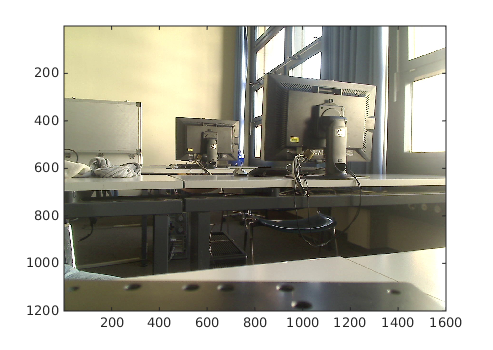
\includegraphics[width=\textwidth]{img/auto}
        \caption{Automatic exposure and gain.}
    \end{subfigure}
    \begin{subfigure}[p]{0.45\textwidth}
        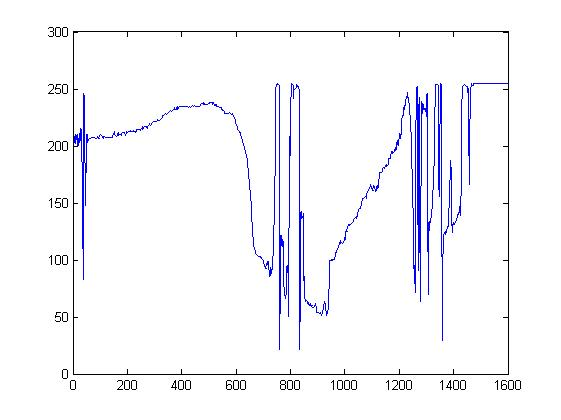
\includegraphics[width=\textwidth]{img/auto_int}
        \caption{Intensity plot at $y=300$.}
    \end{subfigure}
    \centering
    \begin{subfigure}[p]{0.45\textwidth}
        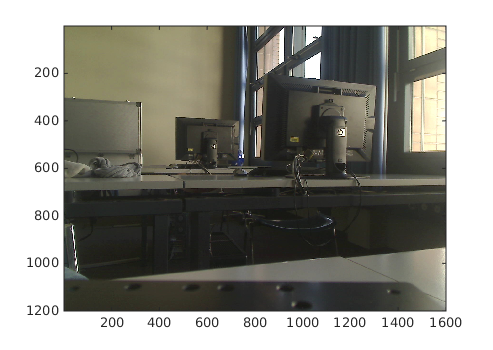
\includegraphics[width=\textwidth]{img/little_sat}
        \caption{Only a couple of pixels are saturated.}
    \end{subfigure}
    \begin{subfigure}[p]{0.45\textwidth}
        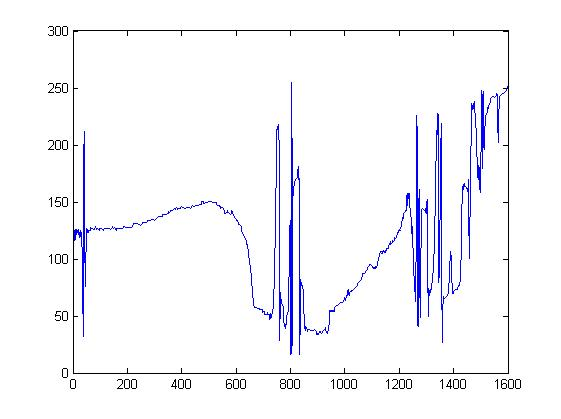
\includegraphics[width=\textwidth]{img/little_int}
        \caption{Intensity plot at $y=300$.}
    \end{subfigure}
    \centering
    \begin{subfigure}[p]{0.45\textwidth}
        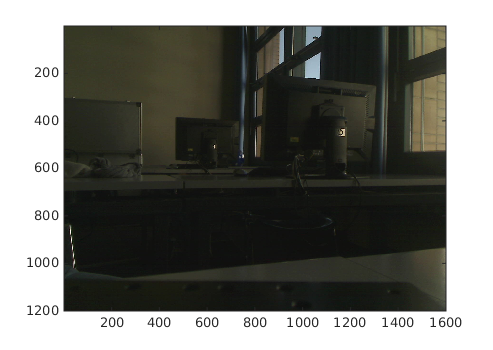
\includegraphics[width=\textwidth]{img/no_sat}
        \caption{No saturation at all.}
    \end{subfigure}
    \begin{subfigure}[p]{0.45\textwidth}
        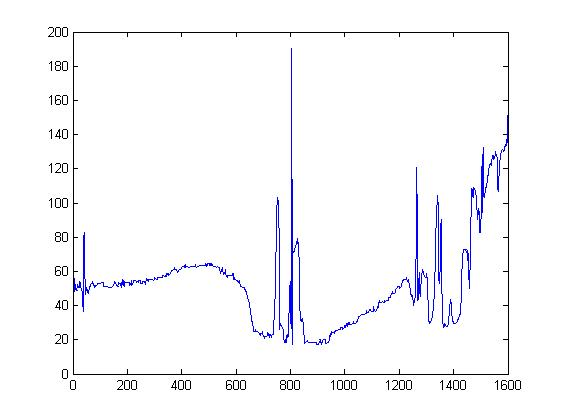
\includegraphics[width=\textwidth]{img/no_sat_int}
        \caption{Intensity plot at $y=300$.}
    \end{subfigure}
    \caption{Comparison of different exposure times.}
\label{fig:saturation}
\end{figure}

\subsection{Procedure to measure the focal length}

First, we measure the magnification at two different focus settings.
For that, we take pictures of a ruler, which gives us the \emph{object size} $s_O$~(figure~\ref{fig:focus_length}).
The \emph{image size} $s_I$ is constant and given by size of the camera sensor.
We then use equation~\ref{equ:magnification} to calculate the magnification.

\begin{figure}[h]
    \centering
    \begin{subfigure}[b]{0.45\textwidth}
        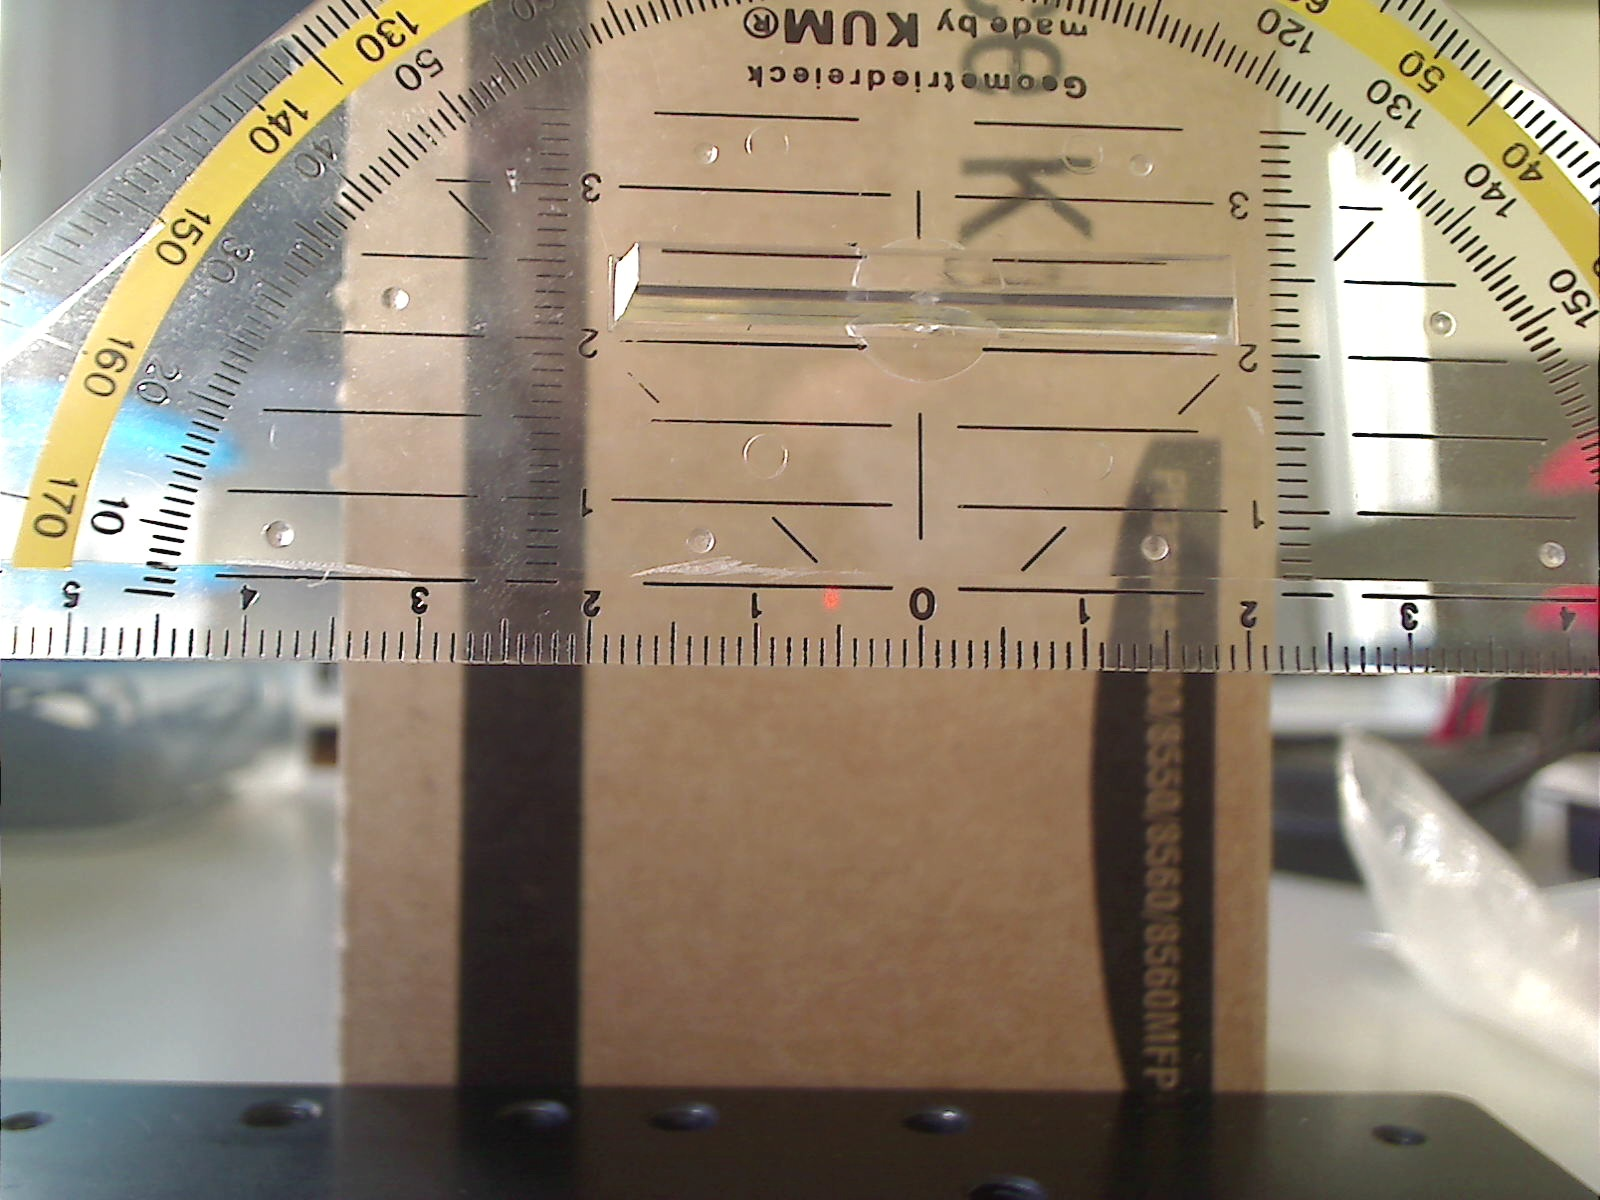
\includegraphics[width=\textwidth]{img/focale1.jpg}
        \caption{Object size of \SI{96}{\milli\meter}}
    \end{subfigure}
    \begin{subfigure}[b]{0.45\textwidth}
        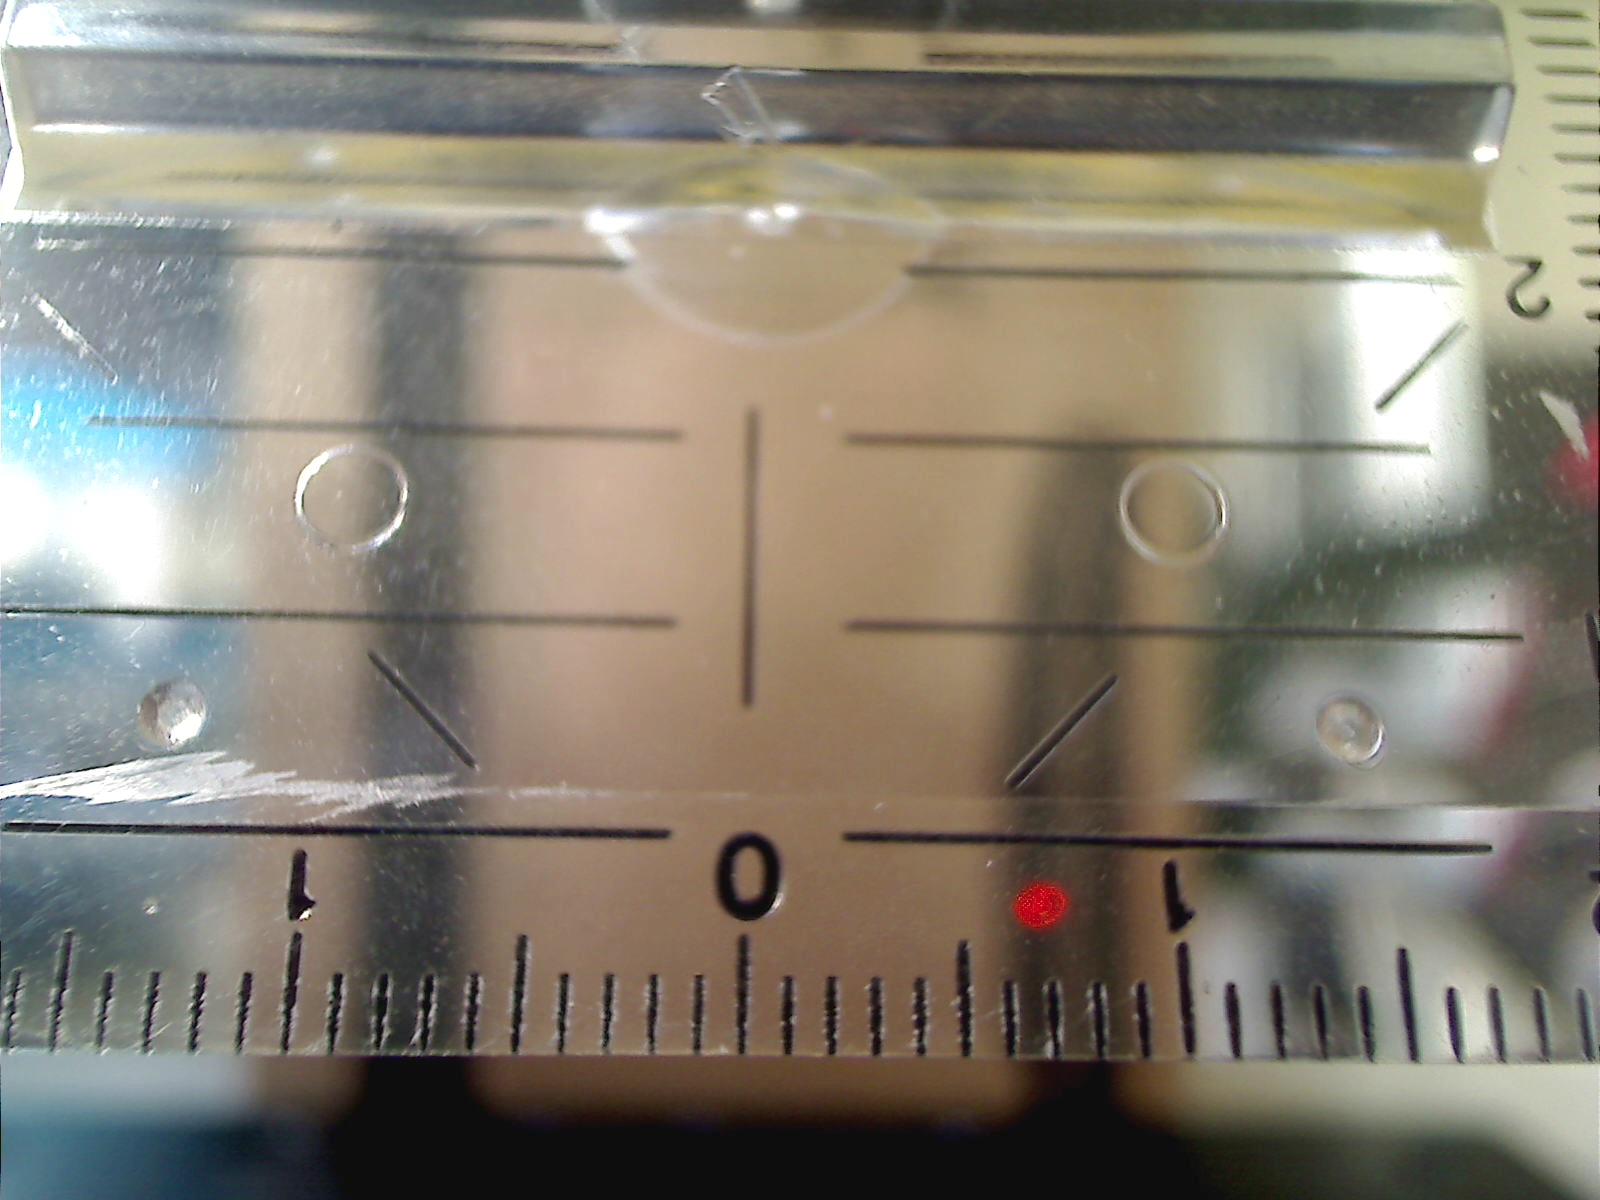
\includegraphics[width=\textwidth]{img/focale2.jpg}
        \caption{Object size of \SI{35.5}{\milli\meter}}
    \end{subfigure}
    \caption{Focusing on a ruler to know the object size.}
\label{fig:focus_length}
\end{figure}

\begin{equation}
    m = \frac{s_I}{s_O}
    \label{equ:magnification}
\end{equation}

We consider the measurement error of the image size $\Delta s_I$ negligible, and calculate the error of the magnification using equation~\ref{equ:magnification_err}.

\begin{equation}
    \Delta m = \frac{s_I}{s_O^2} \Delta s_O
    \label{equ:magnification_err}
\end{equation}

\begin{table}[h]
    \centering
    \begin{tabular}{c r r r r c r r}
        \toprule
        No. & Object size $s_O$ & Image size $s_I$ & $m$ & $\Delta s_O$ & $\Delta s_I$ & $\Delta m$ & $\frac{\Delta m}{m}$ \\
        \midrule
        A & \SI{96}{\milli\meter} & \SI{4.535}{\milli\meter} & \num{0.0472} & \SI{0.25}{\milli\meter} & - & \num{1.23e-4} & 0.25\% \\
        B & \SI{35.5}{\milli\meter} & \SI{4.535}{\milli\meter} & \num{0.128} & \SI{0.25}{\milli\meter} & - & \num{9.00e-4} & 0.70\% \\
        \bottomrule
    \end{tabular}
    \caption{Magnifications for two different foci and their errors.}
\label{tab:magnification}
\end{table}


The focal length is given by equation~\ref{equ:focal_length} with $ d_{IB} - d_{IA} = 0.333 mm $ being the distance we moved the objective (corresponding to one full turn).

\begin{equation}
    f = \frac{d_{IB} - d_{IA}}{m_B - m_A} = \SI{4.1}{\milli\meter}
    \label{equ:focal_length}
\end{equation}

Considering we screwed the objective a full turn with a precision of \SI{10}{\degree} then $\Delta \left(d_{IB} - d_{IA}\right) = \SI{9.25e-3}{\milli\meter}$.

\begin{equation}
    \Delta f = \frac{1}{m_B - m_A} \Delta \left(d_{IB} - d_{IA}\right)
        + \frac{d_{IB} - d_{IA}}{\left(m_B - m_A\right)^2}
        \left(\Delta m_A + \Delta m_B\right) = \SI{0.167}{\milli\meter}
    \label{equ:focal_length_err}
\end{equation}

\begin{equation}
    \frac{\Delta f}{f} = \SI{4.0}{\percent}
    \label{equ:focal_length_err_percent}
\end{equation}

\subsection{Measurement of the field of view}
We measured the object size $s_O = \SI{54.5}{\milli\meter}$ and the distance to the objective $d_O = \SI{46}{\milli\meter}$ with a ruler.
Simple trigonometry yeilds equation~\ref{equ:view_angle}.

\begin{equation}
    \alpha = 2 \arctan{\frac{s_O}{2 d_O}} = \SI{61.3}{\degree}
    \label{equ:view_angle}
\end{equation}

We consider $\Delta s_O = \SI{0.25}{\milli\meter}$ and $\Delta d_O = \SI{0.5}{\milli\meter}$ and calculate the error with equation~\ref{equ:view_angle_err}.

\begin{equation}
    \Delta \alpha = \frac{4 d_O}{s_O^2 + 4 d_O^2} \Delta s_O
    + \frac{4 s_O}{s_O^2 + 4 d_O^2} \Delta d_O = \SI{0.777}{\degree}
    \label{equ:view_angle_err}
\end{equation}

\begin{equation}
    \frac{\Delta \alpha}{\alpha} = \SI{1.27}{\percent}
    \label{equ:view_angle_err_percent}
\end{equation}

\subsection{Measurement of the F\# number}
\subsection{Example from real world}


\section{Discussion and conclusions}
\lipsum[6]
\end{document}
